\chapter{Indledning}

\section{Baggrund}
I Danmark er den demografiske udvikling under stor vækst. Denne skaber en række demografiske sårbarheder, som regeringen, religioneren og kommunerne ikke kan undgå at reagere på. KL har i 2014 lavet en analyserapport "Danmark i forandring", der gennem statistikker fra Danmarks statistik klarlægger forskellige tendenser. I rapporten er der forskellige fremskrivninger, der bygger på gennemsnittet af en række fremskrivningsparametre over de foregående fire år (fra 2010-2014)\footnote{Analyserapport KL}. Fremskrivninger er dermed ikke en prognose, men et billede for, hvordan fremtiden vil se ud, hvis de samme tendenser foreligger. Første kapitel tager fat i befolkningsudviklingen og den demografi udvikling. \\
Konklusionen er, at kommuner udenfor de store byer er præget af flere ældre, færre erhvervsaktive og lave fødselstal. Fra 1980 til 2014 er der blevet knap 10 pct. flere borger i Danmark. Tendensen er, at flere og flere flytter fra yderkommunerne til bykommunerne\footnote{Analyserapport KL figur 1.1 og 1.2 }. Tallene viser at gennemsnitsalderen er voksende. Den er steget med 4 pct. fra 1980 til 2014. Der er dog stor forskel på fordelingen i mellem kommunerne\footnote{Analyserapport KL figur 1.6}. Yderkommunerne har den højste gennemsnitsalder, mens bykommunerne scorer den laveste. Disse tendenser påvirker ældrekvoten, som er en af de store udfordringer. Udviklingen gør, at der stadig er færre personer i den arbejdsdygtige aldre til at forsørge stadig flere udenfor den erhvervsaktive aldre, og dette vil på sigt skabe store problemer, særligt indenfor sundheds- og plejesektoren\footnote{Analyserapport KL tabel 1.1, figur 1.8 og 1.9}. 

Med disse demografiske samt økonomiske udfordringer Danmark står overfor, er det nødvendigt at tænke i andre baner. Sundhed skal leveres på nye måder - på mere smarte og teknologiske måder.        

Telemedicin er derfor for alvor kommet på dagsorden hos regeringen, religionerne og kommunerne. I 2012 udarbejdede disse parter en ambitiøs national handlingsplan for udbredelsen af telemedicin i Danmark\footnote{Udbredelse af telemedicin i hele landet. Digitaliseringsstyrelsen (web)}. Arbejdet med denne handleplan skal give den vigtige erfaring med telemedicin samt give mulighed for parterne at udarbejde fælles modeller for samarbejde, arbejdsgange, økonomiske konsekvenser og øvrige effekter af de konkrete telemedicinske løsninger. Et af de helt klare formål med denne handleplan, er at sikre, at udbredelsen af telemedicin til nye patientgrupper og behandlingsområder vil forløbe hurtigere og mere sikkert i fremtiden. Målet er også at skabe fælles nationale standarder for sundheds-it, så nye telemedicinske løsninger udvikles, så systemerne kan arbejde sammen på tværs\footnote{Telemedicin en nøgle til fremtidens sundhedsydelser}. \\
Digitaliseringsstyrelsen ser også mulighederne for de telemedicinske løsninger og er ved at lave en ny fællesoffentlig digitaliseringsstrategi frem mod 2020, hvor et af pejlemærkerne tager udgangspunkt i den offentlige sektor digitalisering, og som har datadeling, datasikkerhed og it-infrastruktur som temaer \footnote{Kommissorium og målbillede 2020. Digitaliseringsstyrelsen (web)}. Denne strategi skal understøtte de teknologiske muligheder for smartere og mere sikker deling af data mellem borger og offentlige sektor\footnote{målbillede for strategi for digitaliseringen}.\\
Kommunerne har også en strategi, men denne er fokuseret breder - nemlig på telesundhed og ikke telemedicin.

Telesundhed indgår i det overordnede begreb velfærdsteknologi. Telesundhed dækker endvidere begrebet telemedicin\footnote{Kommunernes strategi for telesundhed}. Forholdet mellem de tre begreber er illustreret i figur 1.1. 

\begin{figure}[H]
	\centering
	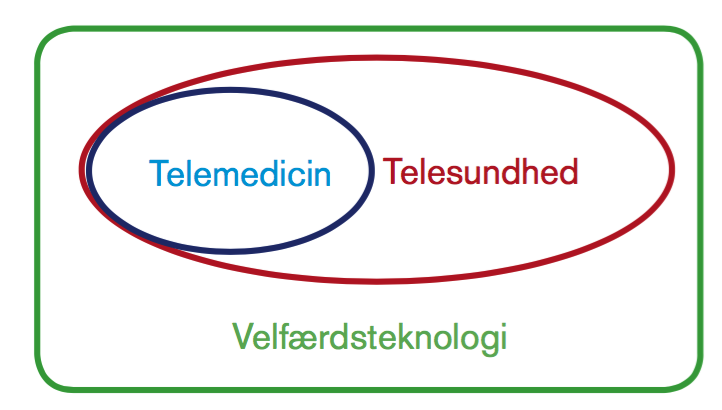
\includegraphics[width=0.8\textwidth]{Figurer/Snip20160426_6}
	\caption{Forholdet mellem velfærdsteknologi, telesundhed og telemedicin \protect\footnotemark}
\end{figure}
\footnotetext{Kommunernes strategi for telesundhed}

I "Kommunernes strategi for telesundhed" defineres telesundhed som brugen af informations- og kommunikationsteknologi til at understøtte, forebygge, behandlende eller rehabiliterende aktiviteter over afstand. Telesundhed tager udgangspunkt i borgeren og borgerens samlede behov for kontakt med sundhedsvæsenet. Derimod er telemedicin mere fokuseret på selve diagnosen og behandlingen borgeren har behov for. Telesundhed fokuserer på borgernes helbred inden, de bliver patienter\footnote{Telemedicin og telesundhed - Sundhedsdatastyrelsen (web)}.

Kommunernes vision med denne strategi er at skabe et bedre grundlag for at borgerne kan mestre eget liv og tilstand og deltage aktivt i egen forbyggelse, behandling og genoptræning, når borgeren selv ønsker det. Et mål er at borgeren ikke skal være begrænset af bestemt tid og sted\footnote{Kommunernes strategi for telesundhed}.

På baggrund af den demografiske udvikling, hvor der vil være færre erhvervsdygtige til at forsørge den stignede ældrekvote, vil telesundhed kunne levere sundhedsydelser på en ny og mere effektivt måde. I hjemmeplejen har man i flere forskellige kommuner forsøgt sig med virtuel hjemmepleje. Viborg kommune har efter et pilotprojekt fra 2013 gode erfaringer med virtuel hjemmepleje og har fra 2014 til 2017 et  udviklings - og forskningsprojekt kørerende\footnote{Virtuel hjemme- og sygepleje. Viborg (web}.  


  


 

 


Telesundhed = Virtuel hjemmepleje. World wide - eksempler hvor det er blevet benyttet og virker. eksempler på kommuner, der har forsøgt sig med virtuel hjemmepleje - samt hvilke løsninger/leverandører. (videnskabelige artikler, er der nogle, der har lavet nogle studier) 
ulemper = infrastruktur.
 

\section{Formål}
Netplan Care og Favrskov Kommune er i gang med et innovationssamarbejde om udviklingen af en kommunal digital velfærdsteknologisk sundhedsstrategi for Telesundhed. 
\\ \\
Telesundhed dækker over digitale velfærdsydelser på mobil- og bredbåndsnettet, hvor sundhedsfaglig dialog og behandling ved brug af den digitale infrastruktur muliggør, at borgere smidigt og omkostningseffektivt kan komme i kontakt med sundhedsvæsenet.    
\\ \\
Video er den mest komplekse løsningskomponent i forhold til telesundhedsløsninger. En af de digitale velfærdsteknologier Favrskov Kommune arbejder med at implementere er Virtuel hjemmepleje, som i høj grad benytter videos som et redskab til kommunikation mellem borger og sundhedsprofessionel. 
\\ \\
Sundhedsteknologistuderende fra Aarhus Ingeniørhøjskole udarbejder i samarbejde med Netplan Care og Favrskov Kommune en Medicinsk Teknologi Vurdering af videobaserede løsninger for Virtuel hjemmepleje. Analysen skal især afdække de teknologiske aspekter samt borgeres reaktioner på video som telesundhedsløsning. Ligeledes vil aspektet om organistionen være i fokus. 

\section{Fokuserede spørgsmål}
\begin{itemize}
	\item Hvilke forudsætninger skal der til for at video fungerer i telesundhedsløsninger? 
	\item Hvilket behov kan video i telesundhedsløsninger dække?
	\item Hvordan er brugernes reaktion og hvad skal man være opmærksom på, opdelt på de sundhedsprofessionelle og borgerne. 
\end{itemize}

